\documentclass[12pt]{article}

\usepackage[a4paper,margin=2cm]{geometry}

\usepackage{amsmath}
\usepackage{amssymb}
\usepackage{mathtools}

\usepackage{listings}

\usepackage{enumerate}
\usepackage{enumitem}

\usepackage{nameref}

\usepackage{xcolor}

\definecolor{codegreen}{rgb}{0,0.6,0}
\definecolor{codegray}{rgb}{0.5,0.5,0.5}
\definecolor{codepurple}{rgb}{0.58,0,0.82}
\definecolor{backcolour}{rgb}{0.95,0.95,0.92}

\lstdefinestyle{mystyle}{
    backgroundcolor=\color{backcolour},
    commentstyle=\color{codegreen},
    keywordstyle=\color{magenta},
    numberstyle=\tiny\color{codegray},
    stringstyle=\color{codepurple},
    basicstyle=\ttfamily\footnotesize,
    breakatwhitespace=false,
    breaklines=true,
    captionpos=b,
    keepspaces=true,
    numbers=left,
    numbersep=5pt,
    showspaces=false,
    showstringspaces=false,
    showtabs=false,
    tabsize=2
}

\lstset{style=mystyle}

\DeclarePairedDelimiter\abs{\lvert}{\rvert}
\DeclarePairedDelimiter\Abs{\lVert}{\rVert}

\usepackage{fancyhdr}

\pagestyle{fancy}
\lhead{\today}
\chead{Exercise 01\\Algorithmic Foundations of Data Science}
\rhead{Tanhim Islam\\Simon Michau\\Til Mohr}

\setlength{\headheight}{50pt}

\begin{document}

\section*{Exercise 1}
We can define the \textit{edit distance} $d_{\text{edit}}(w,w'): \Sigma^2 \rightarrow \mathbb{R}$ as follows. (Let $w=w_1 \dots w_n$ and $w'=w'_1 \dots w'_m$)

\begin{equation*}
	d_{\text{edit}}(w,w') \mapsto
	\begin{cases}
		\abs{w} & \text{if } \abs{w'}=0 \\
		\abs{w'} & \text{if } \abs{w}=0 \\
		d_{\text{edit}}(w_2 \dots w_n, w'_2 \dots w'_m) & \text{if } w_1 = w'_1 \\
		1 + \min
			\begin {cases}
				d_{\text{edit}}(w_2 \dots w_n, w') \\
				d_{\text{edit}}(w, w'_2 \dots w'_m) \\
				d_{\text{edit}}(w_2 \dots w_n, w'_2 \dots w'_m)
			\end{cases}
			& \text{otherwise}
	\end{cases}
\end{equation*}

As this definition of $d_{\text{edit}}$ works by removing at most the first character of each word, we can proof by induction the length of $x,y,z \in \Sigma$, that $d_{\text{edit}}$ is a metric on $\Sigma$:
\begin{itemize}
	\item	Let $\abs{x}=\abs{y}=\abs{z}=0$. Therefore, also $x=y=z$. \\
			Then $0 \leq d_{\text{edit}} = 0$. Thus, Nonnegativity is given. \\
			Since $x=y$, also $d_{\text{edit}}(x,y) = d_{\text{edit}}(y,x)$. Thus, Symmetry is given. \\
			Since $x=y=z$, the Triangle Inequality $d_{\text{edit}}(x,z) \leq d_{\text{edit}}(x,y) + (d_{\text{edit}})(y,z) \Leftrightarrow 0 \leq 0 + 0$ is given.
	\item 	Let $x=x_1 \dots x_n$, $y=y_1 \dots y_m$, and $z=z_1 \dots z_o$, $n,m,o \geq 1$. For $x'=x_2 \dots x_n$, $y'=y_2 \dots y_m$, and $z'=z_2 \dots z_o$ Nonnegativity, Symmetry, and the Triangle Inequality of $d_{\text{edit}}$ is given.
	\item	Since $n,m \geq 1$, the second rule of Nonnegativity, namely $d_{\text{edit}}(x,y) \Leftrightarrow x=y$ does not apply here. \\
			Since all $d_{\text{edit}}(x',y'), d_{\text{edit}}(x',y), d_{\text{edit}}(x,y')$ are non-negative, by definition of $d_{\text{edit}}$, $d_{\text{edit}}(x,y)$ must be non-negative as well. Therefore, the Nonnegativity of $d_{\text{edit}}$ is proven.
	\item	If $x_1 = y_1$, then $d_{\text{edit}}(x,y) = d_{\text{edit}}(x',y') = d_{\text{edit}}(y',x') = d_{\text{edit}}(y,x)$ \\
			If $x_1 \neq y_1$, then
	\item	Triangle Inequality
\end{itemize}

\pagebreak
\section*{Exercise 2}
Result (see \nameref{appendix} for code):
\bigskip

Classification: k=2 Manhattan Distance \\
Test (1, -2, 0): Prediction 1 \\
Test (4, -0.5, 2): Prediction -1 \\
Test (1, 1.5, -2.5): Prediction 0 \\
Test (-2, -1, -2): Prediction 0 \\
Test (-4, -1, -1): Prediction 0
\bigskip

Classification: k=3 Manhattan Distance \\
Test (1, -2, 0): Prediction 1 \\
Test (4, -0.5, 2): Prediction -1 \\
Test (1, 1.5, -2.5): Prediction 1 \\
Test (-2, -1, -2): Prediction -1 \\
Test (-4, -1, -1): Prediction 1
\bigskip

Classification: k=2 Euclidean Distance \\
Test (1, -2, 0): Prediction 1 \\
Test (4, -0.5, 2): Prediction -1 \\
Test (1, 1.5, -2.5): Prediction 1 \\
Test (-2, -1, -2): Prediction 0 \\
Test (-4, -1, -1): Prediction 0
\bigskip

Classification: k=3 Euclidean Distance \\
Test (1, -2, 0): Prediction 1 \\
Test (4, -0.5, 2): Prediction -1 \\
Test (1, 1.5, -2.5): Prediction 1 \\
Test (-2, -1, -2): Prediction 1 \\
Test (-4, -1, -1): Prediction -1
\bigskip

\section*{Exercise 3}
\begin{enumerate}[label=(\alph*)]
	\item	$X_1 \land X_2 \land X_3$ is obviously in $1$-CNF, thus also in $2$-CNF. There exists no satisfiability equivalent formula in $2$-DNF. For this, there would have to be at least two disjunctions of conjunctions of at most 2 literals. Thus, such a formula would be true even if one literal would be false.
	\item	$X_1 \lor X_2 \lor X_3$ is obviously in $1$-DNF, thus also in $2$-DNF. There exists no satisfiability equivalent formula in $2$-CNF. Since such a formula can only have 2 literals in each disjunction, there is no possibility of validating, that the third literal might be true. Therefore, such a formula is not true, when just one literal is true, the others false.
	\item
\end{enumerate}


\section*{Exercise 4}
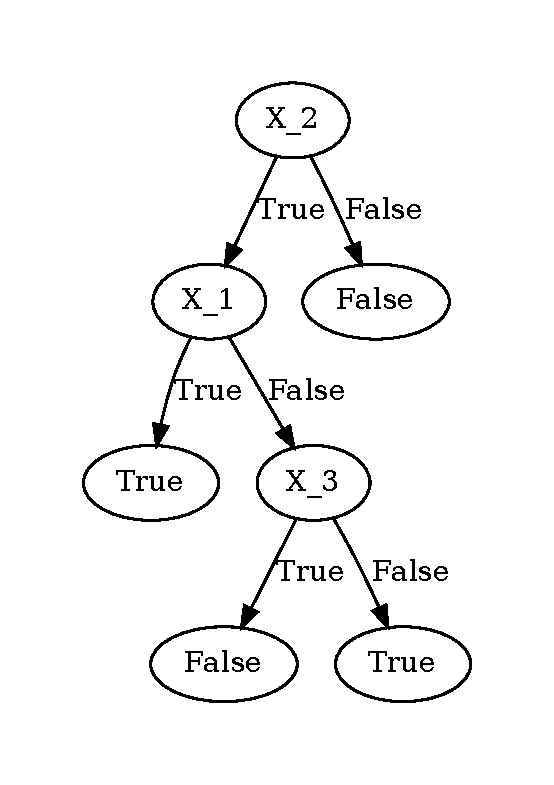
\includegraphics{code/Decision-Tree.gv.pdf} \\
Reasoning (see \nameref{appendix} for code):
\bigskip

Feature Set: $[X_1, X_2, X_3]$ \\
Gains for each feature $[(X_2, 0.5487949406953987), (X_1, 0.04879494069539858), (X_3, 0.04879494069539858)]$ \\
Splitting using feature $X_2$
\bigskip

Feature Set: $[X_1, X_3]$ \\
Gains for each feature $[(X_1, 0.31127812445913283), (X_3, 0.31127812445913283)]$ \\
Splitting using feature $X_1$
\bigskip

Feature Set: $[X_3]$ \\
Gains for each feature $[(X_3, 1.0)]$ \\
Splitting using feature $X_3$ \\

\section*{Exercise 5}
\begin{enumerate}[label=(\alph*)]
	\item	$x_0' = [0, 0, 0, 1, 0]^\top$, since $\langle a,x \rangle = \frac{1}{3} \cdot (3 \cdot 0 + 1 \cdot 0 + 2 \cdot 0 + -2 \cdot 1 + 3 \cdot 0) = -\frac{2}{3}$
	\item	$\langle a,x_1 \rangle + \frac{2}{3} = \frac{1}{3} \cdot (3+1+2-2+3) + \frac{2}{3} = \frac{7+2}{3} = 3 \geq 0$ \\
			$\langle a,x_1' \rangle + \frac{2}{3} = \frac{1}{3} \cdot (3-1-2+2-3) + \frac{2}{3} = \frac{-1+2}{3} = \frac{1}{3} \geq 0$ \\
			Therefore, $x_1,x_1'$ are contained in the same halfspace.
	\item	Let $X \in P$ be a point on the hyperplane. Then the length of the projection of $(x_1 - X)$ is $\frac{\abs{\langle a,x_0 - X \rangle}}{\Abs{a}} = \frac{\abs{\langle a,x_0 \rangle - \langle a,X \rangle}}{\Abs{a}} = \frac{\langle a,x_1 \rangle + b}{\Abs{a}} = \frac{3}{26 + \frac{1}{9}} = \frac{27}{235} \simeq 0.11489$
\end{enumerate}

\section*{Exercise 6}
Since we are in $\mathbb{R}^3$ we can divide the grape by all 3 dimensions twice, thus splitting the grape with 3 strikes into $2^3=8$ pieces. The last strike cannot split the grape by another dimension. We can only split at most 7 pieces in half, thus a maximum of 15 pieces. The swordmasters claims are invalid.

\section*{Appendix}\label{appendix}
\subsection*{Code for Exercise 2}
\lstinputlisting[language=Python]{code/k-nearest-neighbor.py}

\subsection*{Code for Exercise 4}
\lstinputlisting[language=Python]{code/decision-tree.py}

\end{document}